\begin{frame}
\frametitle{Strength of EDM resonance}

\vspace{-0.2cm}
\begin{columns}
	\column{0.5\textwidth}
	\begin{block}{\normalsize \textbf{EDM induced  polarization oscillation,}}
		\begin{itemize}
			\item  can generally be described by 
			\begin{equation}
			p_y(t)  = a \, \sin ( \Omega^{p_y} \, t + \phi_\text{RF}) \,, \nonumber
			\label{eq:initial-slope-from-full-oscillation}
			\end{equation}
			$y$ perpendicular to ring plane.
			
			\item \textbf{EDM resonance strength} defined as ratio of angular frequency $\Omega^{p_y}$ to  orbital angular frequency $\Omega^\text{rev}$\,\textcolor{PineGreen}{\small \cite{PhysRevAccelBeams.23.024601}},
			\begin{equation}
			\varepsilon^\text{EDM} = \frac{\Omega^{p_y}}{\Omega^\text{rev}}\,, \nonumber
			\label{eq:resonance-strength}
			\end{equation}
		\end{itemize}
	\end{block}
	
	\column{0.5\textwidth}
	\begin{figure}
		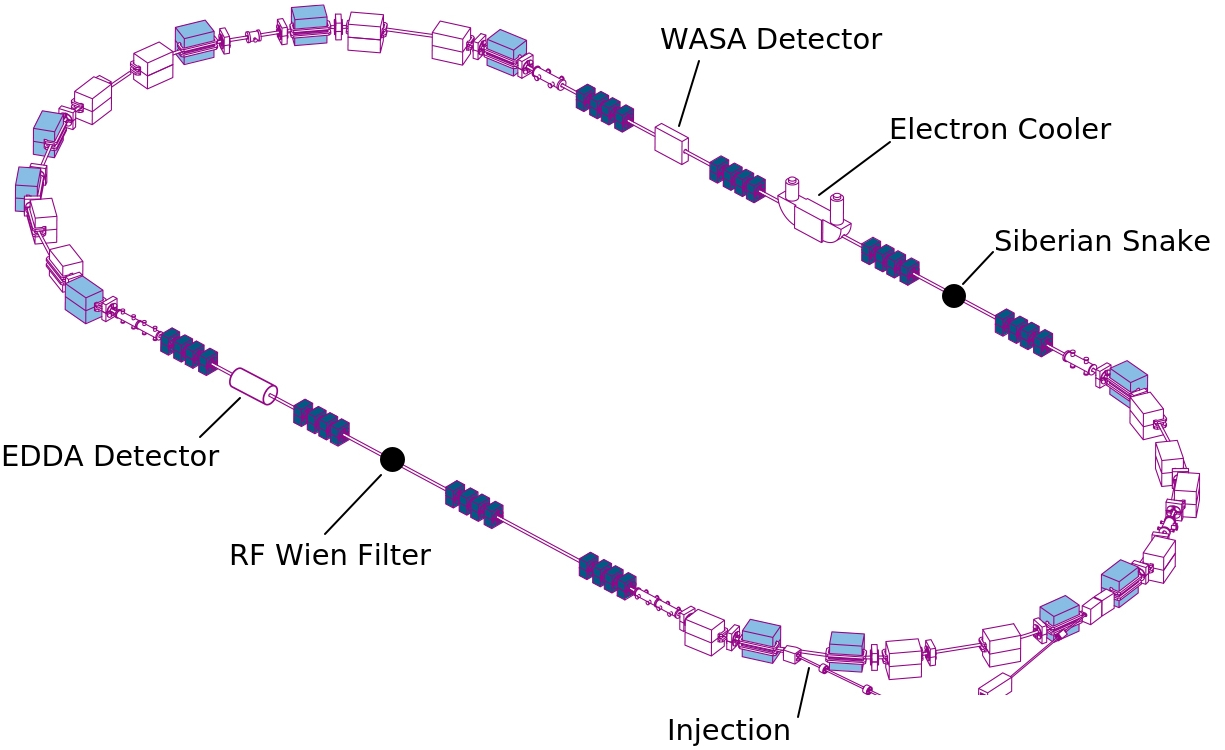
\includegraphics[width=0.95\textwidth]{COSY-landscape.jpg}
	\end{figure}
\end{columns}

\begin{block}{How is the EDM effect actually measured?}
	Two \textit{simultaneously} applied spin rotations, one in each opposite straight section:
	\begin{enumerate}
		\item \textbf{RF Wien filter} magnetic axis ($\vec e_z^\perp$) rotated by small angle $\rightarrow$ generates radial magnetic RF field about which spins precess.
		\item Longitudinal magnetic field of \textbf{Siberian snake}  opposite to Wien filter $\rightarrow$ rotates spins about $\vec e_z$.
	\end{enumerate}
\end{block}

\end{frame}